%% BioMed_Central_Tex_Template_v1.06
%%                                      %
%  bmc_article.tex            ver: 1.06 %
%                                       %

%%IMPORTANT: do not delete the first line of this template
%%It must be present to enable the BMC Submission system to 
%%recognise this template!!

%%%%%%%%%%%%%%%%%%%%%%%%%%%%%%%%%%%%%%%%%
%%                                     %%
%%  LaTeX template for BioMed Central  %%
%%     journal article submissions     %%
%%                                     %%
%%         <14 August 2007>            %%
%%                                     %%
%%                                     %%
%% Uses:                               %%
%% cite.sty, url.sty, bmc_article.cls  %%
%% ifthen.sty. multicol.sty		   %%
%%				      	   %%
%%                                     %%
%%%%%%%%%%%%%%%%%%%%%%%%%%%%%%%%%%%%%%%%%


%%%%%%%%%%%%%%%%%%%%%%%%%%%%%%%%%%%%%%%%%%%%%%%%%%%%%%%%%%%%%%%%%%%%%
%%                                                                 %%	
%% For instructions on how to fill out this Tex template           %%
%% document please refer to Readme.pdf and the instructions for    %%
%% authors page on the biomed central website                      %%
%% http://www.biomedcentral.com/info/authors/                      %%
%%                                                                 %%
%% Please do not use \input{...} to include other tex files.       %%
%% Submit your LaTeX manuscript as one .tex document.              %%
%%                                                                 %%
%% All additional figures and files should be attached             %%
%% separately and not embedded in the \TeX\ document itself.       %%
%%                                                                 %%
%% BioMed Central currently use the MikTex distribution of         %%
%% TeX for Windows) of TeX and LaTeX.  This is available from      %%
%% http://www.miktex.org                                           %%
%%                                                                 %%
%%%%%%%%%%%%%%%%%%%%%%%%%%%%%%%%%%%%%%%%%%%%%%%%%%%%%%%%%%%%%%%%%%%%%


\documentclass[10pt]{article}    



% Load packages
\usepackage{cite} % Make references as [1-4], not [1,2,3,4]
\usepackage{url}  % Formatting web addresses  
\usepackage{ifthen}  % Conditional 
\usepackage{multicol}   %Columns
\usepackage{hhline}
\usepackage[utf8]{inputenc} %unicode support
\usepackage{graphicx}
\usepackage{verbatim}
\usepackage{amsmath}
\usepackage{xspace}
%\usepackage[applemac]{inputenc} %applemac support if unicode package fails
%\usepackage[latin1]{inputenc} %UNIX support if unicode package fails
\urlstyle{rm}
 
 
%%%%%%%%%%%%%%%%%%%%%%%%%%%%%%%%%%%%%%%%%%%%%%%%%	
%%                                             %%
%%  If you wish to display your graphics for   %%
%%  your own use using includegraphic or       %%
%%  includegraphics, then comment out the      %%
%%  following two lines of code.               %%   
%%  NB: These line *must* be included when     %%
%%  submitting to BMC.                         %% 
%%  All figure files must be submitted as      %%
%%  separate graphics through the BMC          %%
%%  submission process, not included in the    %% 
%%  submitted article.                         %% 
%%                                             %%
%%%%%%%%%%%%%%%%%%%%%%%%%%%%%%%%%%%%%%%%%%%%%%%%%                     


%\def\includegraphic{}
%\def\includegraphics{}



\setlength{\topmargin}{0.0cm}
\setlength{\textheight}{21.5cm}
\setlength{\oddsidemargin}{0cm} 
\setlength{\textwidth}{16.5cm}
\setlength{\columnsep}{0.6cm}


%%%%%%%%%%%%%%%%%%%%%%%%%%%%%%%%%%%%%%%%%%%%%%%%%%
%%                                              %%
%% You may change the following style settings  %%
%% Should you wish to format your article       %%
%% in a publication style for printing out and  %%
%% sharing with colleagues, but ensure that     %%
%% before submitting to BMC that the style is   %%
%% returned to the Review style setting.        %%
%%                                              %%
%%%%%%%%%%%%%%%%%%%%%%%%%%%%%%%%%%%%%%%%%%%%%%%%%%
 

%Review style settings
%\newenvironment{bmcformat}{\begin{raggedright}\baselineskip20pt\sloppy\setboolean{publ}{false}}{\end{raggedright}\baselineskip20pt\sloppy}

%Publication style settings
%\newenvironment{bmcformat}{\fussy\setboolean{publ}{true}}{\fussy}

%New style setting

% Begin ...
\begin{document}

\newcommand{\forexample}{e.g.\@\xspace}
\newcommand{\thatis}{i.e.\@\xspace}
\newcommand{\andothers}{et al.\@\xspace}
\newcommand{\kmer}{\ensuremath{k}-mer\xspace}
\newcommand{\kmers}{\ensuremath{k}-mers\xspace}
\newcommand{\tool}{Lighter\xspace}

%%%%%%%%%%%%%%%%%%%%%%%%%%%%%%%%%%%%%%%%%%%%%%
%%                                          %%
%% Enter the title of your article here     %%
%%                                          %%
%%%%%%%%%%%%%%%%%%%%%%%%%%%%%%%%%%%%%%%%%%%%%%

%\title{A Probablistic Space-efficient Method of Obtaining Solid Kmers with An Appliction of Error Correction}
\title{Lighter: fast and memory-efficient error correction without counting}

%%%%%%%%%%%%%%%%%%%%%%%%%%%%%%%%%%%%%%%%%%%%%%
%%                                          %%
%% Enter the authors here                   %%
%%                                          %%
%% Ensure \and is entered between all but   %%
%% the last two authors. This will be       %%
%% replaced by a comma in the final article %%
%%                                          %%
%% Ensure there are no trailing spaces at   %% 
%% the ends of the lines                    %%     	
%%                                          %%
%%%%%%%%%%%%%%%%%%%%%%%%%%%%%%%%%%%%%%%%%%%%%%


\author{Li Song$^1$
  Liliana Florea$^2$
  Ben Langmead$^{*3}$
}

%%%%%%%%%%%%%%%%%%%%%%%%%%%%%%%%%%%%%%%%%%%%%%
%%                                          %%
%% Enter the authors' addresses here        %%
%%                                          %%
%%%%%%%%%%%%%%%%%%%%%%%%%%%%%%%%%%%%%%%%%%%%%%

\maketitle

%%%%%%%%%%%%%%%%%%%%%%%%%%%%%%%%%%%%%%%%%%%%%%
%%                                          %%
%% The Abstract begins here                 %%
%%                                          %%  
%% Please refer to the Instructions for     %%
%% authors on http://www.biomedcentral.com  %%
%% and include the section headings         %%
%% accordingly for your article type.       %%   
%%                                          %%
%%%%%%%%%%%%%%%%%%%%%%%%%%%%%%%%%%%%%%%%%%%%%%


\begin{abstract}
        % Do not use inserted blank lines (ie \\) until main body of text.
\emph{Lighter} is a fast and memory-efficient tool for correcting sequencing errors in high-throughput sequencing datasets.
\tool avoids counting \kmers in the sequencing reads.
Instead, it uses a pair of Bloom filters, one populated with a sample of the input \kmers and the other populated with \kmers likely to be correct based on a statistical test.
As long as the sampling fraction is adjusted in inverse proportion to the dataset's average coverage, the Bloom filter size can be held constant while maintaining near-constant accuracy.
\tool is easily applied to very large sequencing datasets.  It is parallelized, uses no secondary storage, and is both faster and more memory-efficient than competing approaches while achieving comparable accuracy.
\tool is free open source software available from \url{https://github.com/mourisl/Lighter/}.
\end{abstract}


%%%%%%%%%%%%%%%%%%%%%%%%%%%%%%%%%%%%%%%%%%%%%%
%%                                          %%
%% The Main Body begins here                %%
%%                                          %%
%% Please refer to the instructions for     %%
%% authors on:                              %%
%% http://www.biomedcentral.com/info/authors%%
%% and include the section headings         %%
%% accordingly for your article type.       %% 
%%                                          %%
%% See the Results and Discussion section   %%
%% for details on how to create sub-sections%%
%%                                          %%
%% use \cite{...} to cite references        %%
%%  \cite{koon} and                         %%
%%  \cite{oreg,khar,zvai,xjon,schn,pond}    %%
%%  \nocite{smith,marg,hunn,advi,koha,mouse}%%
%%                                          %%
%%%%%%%%%%%%%%%%%%%%%%%%%%%%%%%%%%%%%%%%%%%%%%

% The idea of using a Bloom filter to store the solid k-mers is not new; CUDA-EC does this
% What's our story w/r/t choosing k-mer length?

\section*{Introduction}
The cost and throughput of DNA sequencing have improved rapidly in the past several years \cite{glenn2011field}, with recent advances reducing the cost of sequencing a single human genome at 30-fold coverage to around \$1,000 \cite{1kgenomeforreal}.
With these advances has come an explosion of new software for analyzing large sequencing datasets.
Sequencing error correction is a basic need for many of these tools.
Removing errors at the outset of an analysis can improve accuracy of downstream tools such as variant callers \cite{kelley2010quake}.
Removing errors can also improve the speed and memory-efficiency of downstream tools, particularly for analyses involving de novo assembly with De Bruijn graphs since the graph's size increases with the number of distinct \kmers in the dataset \cite{pevzner2001eulerian, chaisson2004fragment}.

To be useful in practice, error correction software must make economical use of time and memory even when input datasets are extremely large (billions of reads) and when the genome under study is also large (billions of nucleotides).
Several methods have been proposed, covering a wide tradeoff space between accuracy, speed and memory- and storage-efficiency.
SHREC \cite{schroder2009shrec} and HiTEC \cite{ilie2011hitec} build a suffix index of the input reads and locate errors by finding instances where a substring is followed by a character less often than expected.
Coral \cite{salmela2011correcting} and ECHO \cite{kao2011echo} find overlaps among reads and use the resulting multiple alignments to detect and correct errors.
Reptile \cite{yang2010reptile} and Hammer \cite{medvedev2011error} detect and correct errors by examining each \kmer's neighborhood in the dataset's \kmer Hamming graph.

% Citations
% Quake: 149, used in GAGE, assemblathon, 
% SHREC: 68, none seem to be users
% Reptile: 52, no obvious users
% HiTEC: 46, none seem to be users
% ECHO: 37, a handful seem to be users
% Hammer: 35, 
% Coral: 34, no obvious users
% CUDA-EC: 33, no obvious users
% DecGPU: 15
% Musket: 8
% BLESS: 0
% Turtle: 1

The most practical and widely used error correction methods descend from the spectral alignment approach introduced in the earliest De Bruijn graph based assemblers \cite{pevzner2001eulerian, chaisson2004fragment}.
These methods count the number of times each \kmer occurs (its \emph{multiplicity}) in the input reads, then apply a threshold such that reads with multiplicity exceeding the threshold are considered \emph{solid}.
Solid \kmers are unlikely to have been altered by sequencing errors.
\kmers with low multiplicity (\emph{weak} \kmers) are systematically edited into solid \kmers using a dynamic-programming solution to the spectral alignment problem \cite{pevzner2001eulerian, chaisson2004fragment} or, more often, a fast heuristic approximation.
Quake \cite{kelley2010quake}, the most widely used error correction tool, uses a hash-based \kmer counter called Jellyfish \cite{marccais2011fast} to determine which \kmers are solid.
CUDA-EC \cite{shi2010parallel} was the first to use a Bloom filter as a space-efficient alternative to hash tables for counting \kmers and for representing the set of solid \kmers.
More recent tools such as Musket \cite{liu2013musket} and BLESS \cite{heo2014bless} use a combination of Bloom filters and hash tables to count \kmers or to represent the set of solid \kmers.

\emph{Lighter} (LIGHTweight ERror corrector) is also in the family of spectral alignment methods, but differs from previous approaches in that it avoids counting \kmers.
Rather than count \kmers, \tool samples \kmers randomly, storing the sample in a Bloom filter.
\tool then uses a statistical test applied to each position of each read to compile a set of solid \kmers, stored in a second Bloom filter.
These two Bloom filters are the only sizable data structures used by \tool.

\tool's crucial advantage is that its parameters can be set such that the memory footprint and the accuracy of the approach are near-constant with respect to coverage.
That is, no matter how deep the coverage, \tool can allocate the same sized Bloom filters and achieve nearly the same (a) Bloom filter occupancy, (b) Bloom filter false positive rate, and (c) error correction accuracy.
\tool does this without using any disk space or other secondary memory.
This is in contrast to BLESS and Quake/Jellyfish, which use secondary memory to store some or all of the \kmer counts.
\tool's accuracy is comparable to competing tools, as we show both in simulation experiments where false positives and false negatives can be measured, and in real-world experiments where read alignment scores and assembly statistics can be measured.  
\tool is also very simple and fast, faster than all other tools tried in our experiments.
These advantages make \tool quite practical compared to previous counting-based approaches, all of which require an amount of memory or secondary storage that increases with depth of coverage.



%\tool makes a series of three passes over the input reads.  The first pass obtains a sample of the k-mers present in the input reads, storing the sample in a Bloom filter A.  The second pass uses Bloom filter A to identify ``solid'' k-mers and stores these in Bloom filter B.  The third pass uses Bloom filter B to detect and correct errors in the input reads.

%One important way to study a species is to sequence its genome and analyze its DNA. The need to understand the genome stimulates the rapid development of DNA sequencing technologies. The output of the DNA sequencing is usually an enormous volume of short fragments from the genome. With these small fragments, computational biologists are able to design complicated methods to reconstruct the original genome by assembling or to detect the mutations from the known reference genome by aligning.

%The volume of the data is so huge that if we align them to the genome, each position is covered by a bunch of reads which is called the coverage. However, the short fragments are not perfect and usually contain a small number of sequecing errors. This affects one of the most important preprocessing stages for the data --- kmer counting, where a kmer is a nucleutide sequence of size k. If there is no sequencing error, all the kmers are from the genome, which are called solid kmers, and its quantity are bounded by the genome size instead of the coverage. This is not true in practice due to the sequecing errors and if the coverage is high enough, like what the sequecing technology gives us nowadays, the kmers containing sequencing errors will dominate the space consumption. To alleviate the impact from those non-solid kmers, various methods have been proposed, like BFcounter[cite]. These methods still suffer from the problem that the space consumption scales up with the coverage. In this paper, we propose a probablitic methods of obtaining solid kmers whose space complexity does not depend on the coverage.

%One immediate applicaiton using the information of solid kmers is error correction. Error correction is very important for the De Brujin graph based genome assemblers to save the memory usage. There are mainly three categories methods for error correction[cite], and converting all the kmers to solid kmers is one of them and is particularly successful for Illumina reads where the read errors are mainly substitutions. There are currently many programs for error corrections, and some of them are highlighted for their low memory usage, like Musket[cite] and Bless[cite]. With the help of our method of obtainig solid kmers and the bloom filters which is a compact probabilitc data structure, we also propose the program Lighter(LIGHT-weight ERror correction) that can do error correction with very small memory footprint and no extra disk consumption.

\section*{Method}
Lighter's workflow is illustrated in Figure \ref{fig:lighter_framework}. Lighter makes three passes over the input reads.  The first pass obtains a sample of the \kmers present in the input reads, storing the sample in Bloom filter A.  The second pass uses Bloom filter A to identify solid \kmers, which it stores in Bloom filter B.  The third pass uses Bloom filter B and a greedy procedure to correct errors in the input reads.

\begin{figure}[h!]
\begin{center}
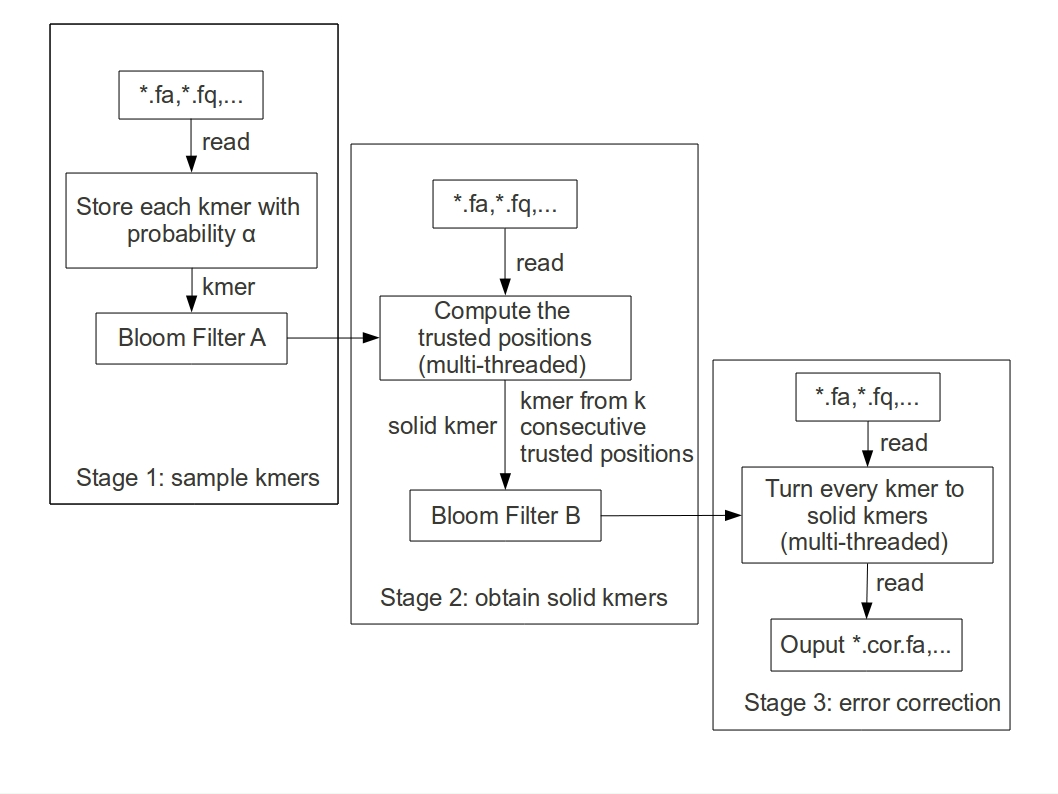
\includegraphics[width=0.75\textwidth]{lighter_framework.jpg}
\caption{The framework of Lighter\label{fig:lighter_framework}}
\end{center}
\end{figure}

\subsection*{Bloom filter}
A Bloom filter \cite{bloom1970space} is a compact probabilistic data structure representing a set.  It consists of an array of $m$ bits, initialized to 0.  To add an object $o$, $h$ independent hash functions $H_0(o), H_1(o),...,H_{h-1}(o)$ are applied.  Each maps $o$ to an integer in $[0, m)$ and the corresponding $h$ array bits are set to 1. To test if object $q$ is a member, the same hash functions are applied to $q$.  $q$ is a member if all corresponding bits are set to 1.  A false positive occurs when the corresponding bits are set to 1 ``by coincidence,'' that is, because of objects besides $q$ that were added previously.  Assuming the hash functions map objects to bit array elements with equal probability, the Bloom filter's false positive rate is approximately $(1-e^{-h\frac{n}{m}})^h$, where $n$ is the number of distinct objects added, which we call the \emph{cardinality}.  Given $n$, which is usually determined by the dataset, $m$ and $h$ can be adjusted to achieve a desired false positive rate.  Lower false positive rates can come at a cost, since greater values of $m$ require more memory and greater values of $k$ require more hash function calculations.  Many variations on Bloom filters have been proposed that additionally permit compression of the filter, storage of count data, representation of maps in addition to sets, etc \cite{tarkoma2012theory}.  Bloom filters and variants thereon have been applied in various bioinformatics settings, including assembly \cite{pell2012scaling}, compression \cite{jones2012compression}, k-mer counting \cite{melsted2011efficient}, and error correction \cite{shi2010parallel}.

By way of contrast, another way to represent a set is with a hash table.  Hash tables do not yield false positives, but Bloom filters are far smaller.  Whereas a Bloom filter is an array of bits, a hash table is an array of buckets, each large enough to store a pointer, key, or both.  If chaining is used, lists associated with buckets incur additional overhead.  While the Bloom filter's small size comes at the expense of false positives, these can be tolerated in many settings including in error correction.

As Figure \ref{fig:lighter_framework} shows, the efficiency of bloom filter affects the running time of Lighter a lot. For a standard Bloom filter, the $h$ hash functions may map $o$ to any places in the bit array. The bit array is usually very large, so all the $h$ accesses will likely to cause cache miss. In [cite], the authors proposed blocked Bloom filter which can decrease the number of cache misses. Given a block size $b$, it will use $H_0(o)$ to decide the start position on the bit array, and then map $H_0(o), H_1(o),...,H_{h-1}(o)$ onto the block starting from that position. It choose $b$ about the size of a cache line, then the $h$ accesses will not cause $h$ cache misses. The drawback of using blocked Bloom filter is that we have to use a bit larger $h$ and $m$ to have the same FPR when using the standard bloom filter. To estimate the FPR of blocked Bloom filter, we can consider each of the possible $m-b+1$ blocks. for the $i$-th block, the FPR within this block is $(b'_i/b)^h$, where $b'_i$ is the number of bits set to 1 in block $i$. So the overall FPR is $\displaystyle\frac{\sum_i (b'_i/b)^h}{m-b+1}$.

In our method, the objects to be stored in the Bloom filters are k-mers.  Because we would like to treat genome strands equivalently for counting purposes, we will always \emph{canonicalize} a \kmer before adding it to, or using it to query a Bloom filter.  A canonicalized \kmer is either the \kmer itself or its reverse complement, whichever is lexicographically prior.

% What do we do with k-mers with ambiguous nucleotides?

\subsection*{Sequencing model}
We use a simple model for the sequencing process (including errors) and for \tool's subsampling.  The sequencing model resembles one suggested previously \cite{melsted2014kmerstream}.  Let $K$ be the total number of \kmers obtained by the sequencer.  We say a \kmer is \emph{incorrect} if its sequence has been altered by one or more sequencing errors.  Otherwise it is \emph{correct}.  Let $\epsilon$ be the fraction of \kmers that are incorrect.  We assume $\epsilon$ does not vary with the depth of sequencing.  The sequencer obtains correct \kmers by sampling independently and uniformly from \kmers in the genome.  Let the number of \kmers in the genome be $G$, and assume all are distinct.  If $\kappa_c$ is a random variable for the multiplicity of a correct \kmer in the input, $\kappa_c$ is binomial with success probability $1/G$ and number of trials $(1-\epsilon)K$: $\kappa_c \sim Binom((1-\epsilon)K, 1/G)$.  Since the number of trials is large and the success probability is small, the binomial is well approximated by a Poisson: $\kappa_c \sim Pois(K(1-\epsilon)/G)$

A sequenced \kmer survives subsampling with probability $\alpha$.  If $\kappa'_c$ is a random variable for the number of times a correct \kmer appears in the subsample, $\kappa'_c \sim Binom((1-\epsilon)K, \alpha/G)$, which is approximately $Pois(\alpha K (1-\epsilon)/G)$.

The model for incorrect \kmers is similar.  The sequencer obtains incorrect \kmers by sampling independently and uniformly from \kmers ``close to'' a \kmer in the genome.  We might define these as the set of all \kmers with low Hamming distance from some genomic \kmer.  If $\kappa_e$ is a random variable for the multiplicity of an incorrect \kmer, $\kappa_e$ is binomial with success probability $1/H$ and number of trials $\epsilon K$: $\kappa_e \sim Binom(\epsilon K, 1/H)$, which is approximately $Pois(K \epsilon / H)$.  It is safe to assume $H \gg G$, but we need not specify $H$ precisely here.  $\kappa'_e \sim Pois(\alpha K \epsilon / H)$ is a random variable for the number of times an incorrect \kmer appears in the subsample.

Others have noted that, given a dataset with deep and uniform coverage, incorrect \kmers occur rarely while correct \kmers occur many times, proportionally to coverage \cite{pevzner2001eulerian, chaisson2004fragment}.

\subsection*{Stages of the method}
\paragraph{First pass.}    In the first pass, Lighter examines each \kmer of each read.  With probability $1 - \alpha$, the \kmer is ignored.  Otherwise, it is canonicalized and added to Bloom filter $A$.

Say a distinct \kmer $K$ occurs a total of $N_K$ times in the dataset.  If subsampling discards all $N_K$ occurrences, the \kmer is never added to $A$ and $A$'s cardinality is reduced by one.  Thus, reducing $\alpha$ can in turn reduce $A$'s cardinality.  Because correct \kmers are more numerous, incorrect \kmers tend to be discarded from $A$ before correct \kmers as $\alpha$ decreases.  Later we show that if $K$ increases but $\alpha K$ is held constant, the cardinality of $A$ and the fraction of correct \kmers in $A$ both remain nearly constant.

The subsampling fraction $\alpha$ is set by the user.  We suggest adjusting $\alpha$ in inverse proportion to depth of sequencing.  For our experiments, we set $\alpha=0.05$ when the average coverage is 70-fold.  That is, we set $\alpha$ to $0.05\frac{70}{C}$ where $C$ is fold coverage.

\paragraph{Second pass.} 
A read position is overlapped by up to $x$ \kmers, $1\le x\le k$, where $x$ depends on how close the position is to either end of the read.
For a position altered by sequencing error, the overlapping \kmers are all incorrect and are unlikely to appear in $A$.
We apply a threshold such that if the number of \kmers overlapping the position and appearing in Bloom filter $A$ is less than the threshold, we say the position is \emph{untrusted}.
Otherwise we say it is \emph{trusted}.
Each instance where the threshold is applied is called a \emph{test case}.
When one or more of the $x$ \kmers involved in two test cases differ, we say the test cases are distinct.

Let $P^*(\alpha)$ be the probability an incorrect \kmer appears in $A$, taking the Bloom filter's false positive rate into account.  If random variable $B_{0,x}$ represents the number of \kmers appearing in $A$ for an untrusted position overlapped by $x$ \kmers, $B_{e,x} \sim Binom(x,P^*(\alpha))$.  We define thresholds $y_x$, for each possible value of $x$ in $[1, k]$.  Each $y_x$ is the minimum integer such that $p(B_{0,x}\le y_x - 1)\ge 0.995$.

Initially we ignore false positives and model the probability of a sequenced a \kmer having been added to $A$ as $P(\alpha)=1-(1-\alpha)^{f(\alpha)}$.  We define $f(\alpha)=max\{2,0.1/\alpha\}$.  That is, we assume the multiplicity of a weak \kmer is at most $f(\alpha)$, which will often be a conservative assumption, especially for small $\alpha$.  It is also possible to define $P(\alpha)$ in terms of random variables $\kappa_e$ and $\kappa'_e$, but we avoid this for simplicity.

A property of this threshold is that when $\alpha$ is small, $P(\alpha/z)=1-(1-\alpha/z)^{0.1z/\alpha}\approx 1-(1-\alpha)^{0.1/\alpha}=P(\alpha)$, where $z$ is a constant greater than 1 and we use the fact that $(1-\alpha/z)^z\approx 1-\alpha$.

For $P^*(\alpha)$, we additionally take $A$'s false positive rate into account.  If the false positive rate is $\beta$, then $P^*(\alpha)=P(\alpha)+\beta-\beta P(\alpha)$.

%Let $m(r)$ denote \kmer $r$'s multiplicity.  Let $P(\alpha, m(r))$ be the probability that $r$ is added to Bloom filter A given sampling rate $\alpha$:
%$$P(\alpha, m(r)) = 1-(1-\alpha)^{m(r)}$$

%When we query Bloom filter $A$, whether we get a positive response depends both on $P(\alpha, m(r))$ and on the filter's false positive rate, which we call $\beta$.  The probability $P^*(\alpha, m(r))$ of getting a positive response when querying for $r$ in $A$ is:

%$$P^*(\alpha, m(r))=P(\alpha, m(r))+\beta-P(\alpha, m(r))\beta$$

%Say $\gamma$ is the expected multiplicity of a correct \kmer.  We call a \kmer $r$ weak if $m(r)$ is much less than $\gamma$. Specifically, we say $r$ is weak if $m(r) \leq \gamma'$, where $\gamma'=\gamma/c$ and $c$ is a constant we must choose. We can bound the probability that a weak \kmer is added to Bloom filter A given sampling rate $\alpha$:

%$$P(\alpha, 1) \leq P_{weak}(\alpha) \leq P(\alpha, \gamma')$$

%The lower bound corresponds to the case where all weak \kmers have multiplicity 1 and the upper bound corresponds to the case where all weak \kmers have multiplicity $\gamma'$.  Additionally taking false positive rate into account, we can bound the probability $P^*_{weak}(\alpha)$ that the Bloom filter gives a positive response when queried with a weak \kmer:

%$$P^*(\alpha, 1) \leq P^*_{weak}(\alpha) \leq P^*(\alpha, \gamma')$$

%In the following we conservatively assume $P_{weak}(\alpha) = P(\alpha, \gamma')$ and $P^*_{weak}(\alpha) = P^*(\alpha, \gamma')$.


%:  above by $P(\alpha, \gamma')$ and below by .

%For the \kmers containing sequencing errors, we will call it true weak kmers. In practice, the multiplicity of most true weak \kmers grows much slower when we increase $\gamma$ namely increasing the coverage. So $\gamma'$ will overestimate the mulitplicity of true weak \kmers a lot. 

 %To determine whether a position is incorrect, we perform a one-tailed hypothesis test where the null hypothesis is that all overlapping \kmers are weak.  For a weak \kmer, a positive response from Bloom filter A happens with probability $P^*(\alpha, \gamma')$ (conservatively), and the number of overlapping \kmers yielding a positive response follows a binomial distribution with success probability $P^*(\alpha, \gamma')$ and number of trials $x$.  Let $y \leq x$ be the actual number of \kmers overlapping the read position that appear in A and let $y'$ be the minimum integer value for $y$ such that the hypothesis test P value is less than 0.005.  If $y \geq y'$, we reject the null hypothesis and the read position is called \emph{trusted}, otherwise it is called \emph{untrusted}. 

%Framing the problem as a hypothesis test is convenient since it naturally handles the case where $x<k$.  $y'$ thresholds can be pre-calculated for efficiency.

%A one-tail hypothesis testing. The null hypothesis is that this position is wrong and the p-value can be get from test again $(x,P^*(\alpha, \gamma'))$ using the actual number of kmers in $A$ containing that position. We use $y$ to denote this actual number of kmers. In our method, suppose $y'$ is the first number whose p-value is smaller than 0.005, if $y>y'$, we reject the null hypothes and the position is trusted. The benefit of using hypothesis testing instead of using a fixed threshold is that we can handle the case where $x<k$ in a consistent way and it can tolerate the ill-chosen $\alpha$. Notice that, the position near the left and right boundary or near an error may never be trusted.

Once all positions in a read have been marked \emph{trusted} or \emph{untrusted} using the threshold, we find all instances where $k$ trusted positions appear consecutively.  The \kmer made up by those positions is added to Bloom filter $B$.

%After marking each positions, if there are consecutive k trusted positions, we store the corresponding kmer, which is likely a solid \kmer, in another bloom filter $B$. Because these kmers are likely from the real genome, the size of $B$ also only depends on the genome size. 

\paragraph{Third pass.} 
In the third pass, \tool applies a simple, greedy error correction procedure similar to that used in BLESS \cite{heo2014bless}.
A read $r$ of length $|r|$, contains $|r|-k+1$ \kmers.
$k_i$ denotes the \kmer starting at read position $i$, $1\le i\le|r|-k+1$.
We first identify the longest stretch of consecutive \kmers in the read that appear in Bloom filter $B$.
Let $k_b$ and $k_e$ be the \kmers at the left and right extremes of the stretch.
If $e < |r|-k+1$, we examine successive \kmers to the right starting at $k_e+1$.
For a \kmer $k_i$ that does not appear in $B$, we assume the nucleotide at offset $i+k-1$ is incorrect.
We consider all possible ways of substituting for the incorrect nucleotide.
We try each possible substitution, then count how many consecutive \kmers starting with $k_i$ appear in Bloom filter $B$.
We choose the substitution that creates the longest stretch of consecutive \kmers in $B$.
If more than one candidate substitution is equally good, we call position $i+k-1$ ambiguous and resume the rightward scan at \kmer $k_i+k$.
The procedure is illustrated in Figure \ref{fig:error_correction}.  If $k_b$ is not the leftmost \kmer in the read, we apply a similar procedure moving leftward.

\begin{figure}[h!]
\begin{center}
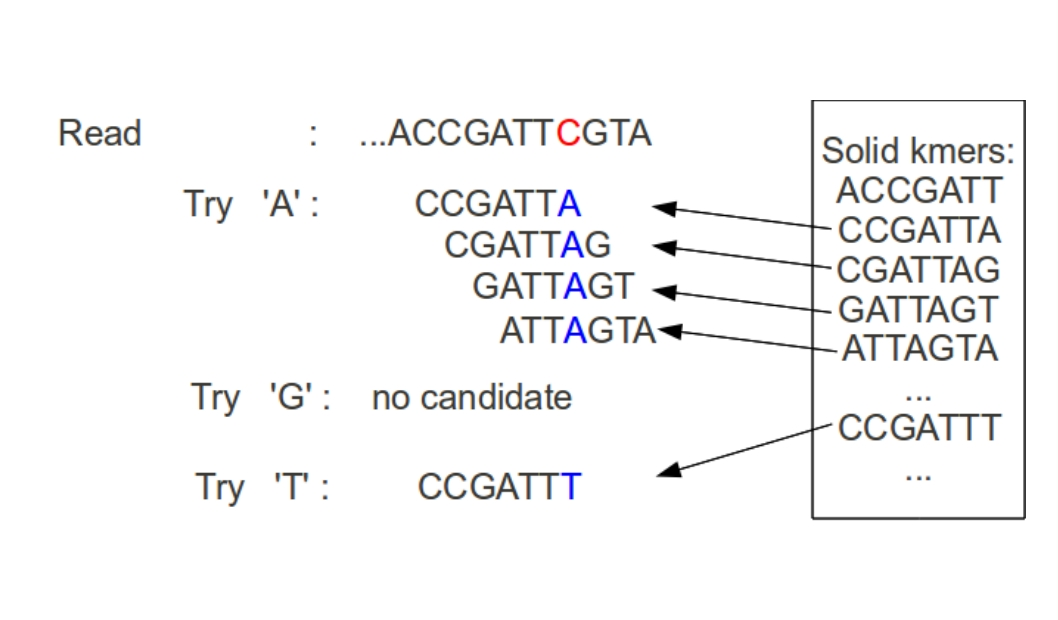
\includegraphics[width=0.75\textwidth]{ErrorCorrection.jpg}
\caption{An example of the greedy error correction procedure.  \kmer CCGATTC does not appear in Bloom filter $B$, so we attempt to substitute a different nucleotide for the C shown in red.  We select A since it yields the longest stretch of consecutive \kmers that appear in Bloom filter $B$.  \label{fig:error_correction}}
\end{center}
\end{figure}

% BTL: I don't understand the following
If the error is located near the end of the read, for each candidate substitution, we will extend reads using the kmer reported in Bloom filter $A$ by one path that has the least lexicographical order. Thus we can solve some ties that are more likely to happend near the end of a read due to insufficient extension. 

\subsection*{Scaling with coverage}
\tool's accuracy is near-constant as the depth of sequencing $K$ increases and its memory footprint is held constant.  The basic idea is that as $K$ increases, we adjust $\alpha$ in inverse proportion.  That is, we hold $\alpha K$ constant.  For concreteness, consider two scenarios: scenario I, where coverage is $K_1$ and subsampling fraction is $\alpha_1$, and scenario II where coverage is $K_2=z K_1$ and subsampling fraction is $\alpha_2 = \alpha_1 / z$.

\paragraph{Contents of Bloom filter A.} The occupancy of Bloom filter $A$, as well as the fraction of correct \kmers in $A$, are approximately the same in both scenarios.  This follows from the fact that $\kappa'_c ~ \sim Pois(\alpha K (1 - \epsilon) / G)$, $\kappa'_e \sim Pois(\alpha K \epsilon / H)$, and $\alpha K$, $\epsilon$, $G$, and $H$ are constant across scenarios.  This is also supported by our experiments, as seen in Table \ref{table:bloom_occupancy_coverage}.  Because the occupancy does not change, we can hold the Bloom filter's size constant and achieve the same false positive rate.

% show that false positive of Bloom filter $A$ stays almost constant. Suppose we have two scenarios, in scenario I, the sequencer outputs $K_1$ \kmers and in scenario II, the sequencer outputs $zK_1$ \kmers. If we set $\alpha$ to be $\alpha_1$ in scenario I, then $\alpha_2=\alpha_1/z$ in scenario II. As a result, the distribution of $\kappa'_c$ and $\kappa'_e$ do not change in scenario II and are $Pois(\alpha_1(1-\epsilon)K_1)$ and $Pois(\alpha_1\epsilon K_1 / H)$ repsectively. The number of correct \kmer get stored in Bloom filter $A$ is $Gp(\kappa'_c\ge 1)$ and the number of incorrector \kmer stored in Bloom filter $A$ is $Hp(\kappa'_e\ge 1)$. These two numbers are the same in scenarios I and II, thus the occupancy rate and the false positive rate of Bloom filter $A$ stays almost the same.

\paragraph{Accuracy of trusted / untrusted classifications.}
Also, if a read position and its neighbors within $k-1$ positions on either side are error-free, then the probability it will be called trusted does not change between scenarios.  We mentioned that when $\alpha$ is small, $P(\alpha_1) \approx P(\alpha_1/z) = P(\alpha_2)$.  We also showed that the false positive rate of the bloom filter is approximately constant between scenarios, so $P^*(\alpha_1) \approx P^*(\alpha_1/z) = P^*(\alpha_2)$.  Thus, the thresholds $y_x$ will also remain unchanged.
$p_c=(p(\kappa'_c\ge 1))/(p(\kappa_c\ge 1))$ is the probability a correct \kmer is in the subsample given that it was sequenced.
$p_c=(1-e^{-\alpha(1-\epsilon) K/G})/(1-e^{-(1-\epsilon) K/G})\approx 1-e^{-\alpha(1-\epsilon)K/G}$, since $(1-\epsilon)K/G$ is large.
$p_c$ is constant across scenarios since $\alpha K$, $\epsilon$, and $G$ are constant.
Since $p_c$ is constant, the parameters of the $B_{e,x}$ distribution are constant and the probability a correct position will be called trusted is also constant.
%If $B_c$ is a random variable for the number of correct \kmers out of $x$ covering a position that appear in Bloom filter $A$, then $B_c \sim Binom(x, p_1+\beta-\beta p_1)$.
%Moreover, the number of different test cases does not change and the overall positions that get classified as trusted is almost the same when changing the coverage.

Now we consider an incorrect read position.  We ignore false positives from Bloom filter $A$ for now.
$p_e = p(\kappa'_e\ge 1)/p(\kappa_e\ge 1) = (1-e^{-\alpha\epsilon K/H})/(1-e^{-\epsilon K/H})$ is the probability an incorrect \kmer is in the subsample given that it was sequenced.
Since $\epsilon K/H$ is close to 0, $e^{-\epsilon K/H}\approx 1-\epsilon K/H$ and $p_e \approx (\alpha \epsilon K/H)/(\epsilon K/H)=\alpha$.
Say an incorrect read position is covered by $x$ \kmers; if $B_{e,x}$ is a random variable for the number of \kmers overlapping the position that appear in Bloom filter $A$, then $B_{e,x} \sim Binom(x, p_e) \approx Binom(x, \alpha)$.  The probability of falsely trusting a position is therefore: 
$p(B_{e, x}\geq y_x)=\sum_{i=y_x}^x \binom{x}{i} p_e^i(1-p_e)^{x-i} \approx \sum_{i=y_x}^x \binom{x}{i} \alpha^i(1-\alpha)^{x-i}$.  If we omit the $(1-\alpha)^{x-i}$ term in the sum, what remains is an upper bound, \thatis $\sum_{i=y_x}^x \binom{x}{i} \alpha^i(1-\alpha)^{x-i} \leq \sum_{i=y_x}^x \binom{x}{i} \alpha^i$.  Since $\alpha_2 = \alpha_1/z$, the upper bound in scenario II is lower by a factor of at least $1/z$ relative to the upper bound in scenario I.  So an upper bound on the probability of labeling an incorrect position as trusted decreases by a factor of at least $z$.  When $K$ increases, the number of distinct test cases for incorrect positions increases by a factor of at most $z$.  Thus, we expect the total number incorrect positions labeled as trusted to remain approximately constant.

When $\alpha$ is small, the false positive rate $\beta$ may dominate the probability $p_e$.  In practice, however, the false positive rate is usually small enough that the probability of a incorrect position being labeled as trusted due to false positives is extremely low.  For example, for many of the experiments reported in this study, the k-mer length $k=17$, the false positive rate of Bloom A $\approx 0.004$, the threshold $y_{2k-1} = 6$, and $\alpha = 0.05$.  In this situation, $p(B_{e, x}\geq y_x) \approx 5 \cdot 10^{-11}.$

The above is not an exhaustive analysis, since we have not examined the case where a read position is error-free but not all of its neighbors within $k-1$ positions on either side are error-free.  In this case, whether the threshold is passed depends chiefly on the whereabouts of the nearby errors.

\paragraph{Contents of Bloom filter B.}

Given the analysis in the previous section, we expect that the collection of \kmers drawn from the stretches of trusted positions in the reads will not change much across scenarios and, therefore, the contents of Bloom filter $B$ will not change much.  This conclusion is also supported by our experiments, as seen in Table \ref{table:bloom_occupancy_coverage}.

%Next we show that the number of positions that contain error and are falsely set as trusted position does not cause trouble. For simplicity, we ignore $\beta$, the affect of the false responses from the Bloom filter $A$, for now. Let $p_2=\frac{p(\kappa'_e\ge 1)}{p(\kappa_e\ge 1)}$. And the number of sampled \kmers covering this position is roughly a binomial distribution $B_2\sim Binom(x, p_2)$. In general, $p_2=\frac{1-e^{-\alpha\epsilon K/H}}{1-e^{-\epsilon K/H}}$. Since $\epsilon K/H$ is very close to 0, $e^{-\epsilon K/H}\approx 1-\epsilon K/H$. So $p_2\approx \frac{\alpha \epsilon K/H}{\epsilon K/H}=\alpha$. In sceanrio I, $p_2=\alpha_1$; and in scenario II, $p_2=\alpha_1/z$.

%Another perspective to get is conclusion is that because the total number of weak kmers get stored in Bloom filter $A$ is constant and the number of different test cases increase, for each test case the number of \kmers we retrieved from Bloom filter $A$ will decrease.

%When $\alpha$ gets too small, $\beta$ may dominant the probability. However, in that case, the probability of $B_2\ge y'$ is extremely small, so it does not cause trouble at that time. For example, in this paper, $\beta$ is less than $0.004$ and the threshold $y'$ is 6 when $\alpha\le 0.05$ and the \kmer size is $17$. Considering the binomial distribution $B'_2\sim Binom(x, 0.004)$, the probability $p(B'_2\ge 6)$ is about $5*10^{-11}$. 

%Therefore, the number of \kmers coming from the consecutive trusted positions does not increase which means there is no need to increase the size of Bloom filter $B$ when increasing coverage. Also, the analysis showed that the ability of capturing solid kmers remains almost the same when we change $\alpha$ linearly. 

\subsection*{Quality score}
Lighter can also use base quality values, essentially by allowing a low quality value to ``veto'' a trusted position.  First, \tool scans the first 1 million reads in the input, recording the quality value at the last position in each read.  \tool then chooses the 5th-percentile quality value; that is, the value such that 5\% of the values are less than or equal to it.  When Lighter decides whether a position is trusted or not, if its quality score is less than the 5th-percentile value, then call it untrusted regardless of how many of the overlapping \kmers appear in Bloom filter $A$.

\subsection*{Parallization} 
As shown in Figure \ref{fig:lighter_framework}, Lighter works in three stages: sampling \kmers, obtaining solid kmers and error correction. For the sampling kmers stage, because $\alpha$ is very small, most of the time is spent on scanning the reads namely reading the files. As a result, the overhead of parallilize this part will dominate the benefits, so we decide to remain this stage serial. In the second stage, each thread will handle different reads independently. Reading bloom filter in parallel is very efficient since there is no data race. When a thread find a solid kmer, it firstly tests whether this kmer is stored in table B or not. If this kmer is not in table B, then we write this kmer into the table. In this way, we can avoid many writing locks for table B because a solid kmer shows up many times. The thrid stage can parallized embarrsingly.

\section*{Evaluation}
\subsection*{Simulated data set}
We compared the our result with other released programs, Quake[cite], Musket[cite] and Bless[cite]. We use Mason[cite] to generate a set of data sets with ecoli as the reference genome. The K12 strain of ecoli is fully sequenced and has the decent length for us to generated different scenarios easily. The \kmer size is 17 for all the programs.

In the simulated data set, we considered the coverage of $35$x, $75$x, $140$x, and the average error rate of $1\%$ and $3\%$. So there are totally 6 data sets. Because Mason can also specifiy the error rate of the first and the last base repsectively, suppose the average error rate is $e$, we set the error rate of the first base to $e/2$ and the error rate of the last base is $3e$. This setting is more realistic than a uniform error rate model. 
%TODO: define recall,...

We say a base is true positive(TP) if we identify the error and correct it into the right one; a base is false positive(FP) if we correct an original error-free base; a base is false negative(FN) if it is wrong and we either fail to detect its error or we make a wrong correction. As tradition[cite], we use four measurement to evaluate the error correction methods: recall=TP/(TP$+$NP), precision=TP/(TP$+$FP), F-score=2$\times$recall$\times$precision/(recall$+$precision) which is a kind of average of recall and precision and Gain=(TP-FP)/(TP+FN) which measure the benefit of using error correction.

% Insert the table here.
\mbox{
\begin{tabular}{|c|c|c|c|c|c|c|c|}\hline
Coverage &	& \multicolumn{2}{|c|}{$35\times$}  & \multicolumn{2}{|c|}{$70\times$} & \multicolumn{2}{|c|}{$140\times$} \\ \hline
Error rate & & $1\%$ & $3\%$ & $1\%$ & $3\%$ & $1\%$ & $3\%$ \\ \hhline{|=|=|=|=|=|=|=|=|}
	& quake	& 89.59	& 48.77	& 89.64	& 48.82	& 89.59	& 48.78 \\ \cline{2-8}
Recall	& musket	& 92.61	& 92.04	& 92.60	& 92.05	& 92.60	& 92.03 \\ \cline{2-8}
	& bless	& 98.68	& 97.29	& 98.69	& 97.48	& 98.65	& 97.47 \\ \cline{2-8}
	& lighter	& \textbf{99.42}	& \textbf{98.03}	& \textbf{99.36}	& \textbf{98.93} & \textbf{99.39}	& \textbf{98.99} \\ \hhline{|=|=|=|=|=|=|=|=|}
	& quake	&\textbf{99.99}	& \textbf{99.99}	& \textbf{99.99}	& \textbf{99.99}	& \textbf{99.99}	& \textbf{99.99} \\ \cline{2-8}
Precision	& musket	& 99.78	& 99.63	& 99.78	& 99.63	& 99.78	& 99.63 \\ \cline{2-8}
	& bless	& 98.90	& 98.59	& 98.88	& 98.62	& 98.88	& 98.61 \\ \cline{2-8}
	& lighter	& 99.10 & 99.14	& 99.08	& 99.18	& 99.07	& 99.18 \\ \hhline{|=|=|=|=|=|=|=|=|}
	& quake	& 94.51	& 65.56	& 94.54	& 65.61	& 94.51	& 65.57 \\ \cline{2-8}
F-score	& musket	& 96.06	& 95.68	& 96.05	& 95.69	& 96.05	& 95.68 \\ \cline{2-8}
	& bless	& 98.79	& 97.94	& 98.78	& 98.04	& 98.77	& 98.04 \\ \cline{2-8}
	& lighter	& \textbf{99.26}	& \textbf{98.58}	& \textbf{99.22}	& \textbf{99.06}	& \textbf{99.23}	& \textbf{99.09} \\ \hhline{|=|=|=|=|=|=|=|=|}
	& quake	& 89.58	& 48.76	& 89.64	& 48.82	& 89.59	& 48.78 \\ \cline{2-8}
Gain	& musket	& 92.40	& 91.70	& 92.39	& 91.71	& 92.39	& 91.69 \\ \cline{2-8}
	& bless	& 97.58	& 95.90	& 97.57	& 96.11	& 97.54	& 96.09 \\ \cline{2-8}
	& lighter	& \textbf{98.52}	& \textbf{97.17}	& \textbf{98.44}	& \textbf{98.12}	& \textbf{98.46}	& \textbf{98.18} \\ \hhline{|=|=|=|=|=|=|=|=|}

\end{tabular}
}

The $\alpha$ value for the $35\times$, $70\times$, $140\times$ is $0.1$, $0.05$ and $0.025$ respectively. 

For Quake, we only measured the performance of the reported reads. Because Quake trimmed the untrusted tail of a read and throw away unfixable reads, it has a particularly high precision. But even if we only count the original errors in those reported reads, its sensitivity is very low. Lighter is among the best on different measurement and scenarios. This shows that our sampling method is able to distinguish most solid and weak kmer, and the error correction method is very effective.

We can show Lighter can achieve near constant space usage if the portion of set bits, namely occupancy rate, in the bloom filters stays almost the same. And this is true as shown in Table \ref{table:bloom_occupancy_coverage} given different coverages using simulated data set with 1\% error rate. When the coverage is very low, the occupancy rate in table $B$ is significant lower. This is because that when the coverage is very low, the count of the solid kmers is not very different from the weak kmers and the binomial test fails no matter how the $\alpha$ is set.

\begin{table}
\begin{tabular}{|c|c|c|}\hline
Coverage & Table A & Table B \\ \hline
$10\times$	& 41.563  &	19.843 \\ \hline
$20\times$	& 41.555  &	32.765 \\ \hline
$35\times$ & 41.555	& 33.802 \\ \hline
$70\times$ & 41.580	& 33.906 \\ \hline
$140\times$ & 41.577 & 33.881  \\ \hline
$280\times$ & 41.571 & 33.903 \\ \hline
\end{tabular}
\caption{Occupancy rate(\%) for each table for different coverages\label{table:bloom_occupancy_coverage}}
\end{table}

To further test the performance of Lighter, we showed how many kmers from the reference genome is stored in table $B$. We used the simulated data with $70$x coverage and $1\%$ error rate. There are totally 4,553,699 distinct kmers from the genome on one strand, and 4,553,653 of them are in table $B$ which is almost all of them. We lose some kmers from the genome mostly due to the low coverage at the two ends of the chromosome.

The 6 simulated data sets are for haploid case, there are many species with a pair of chromosome in a cell, like human. Here we consider the case of diploid. We still use the e.coli genome as the reference genome and then introduce $0.1\%$ SNPs to generate the second reference genome. Mason then will sample the same amount of reads from the two genomes, totally form an $70$x coverage data set. There are 159,117 kmers containing the SNP position from one strand, and table $B$ holds 158,987 of them. Though the performance is not as good as haploid case, it still hold almost all of them. 

% test the performance of alpha
\subsubsection*{Effect of $\alpha$}
The sampling rate $\alpha$ is the key in Lighter which ensures the near constant space complexity. We did an evaluation on the simulated data set with $35\times$ coverage and $1\%$ error rate. The result is shown in Figure \ref{fig:alpha}.

\begin{figure}[h!]
\begin{center}
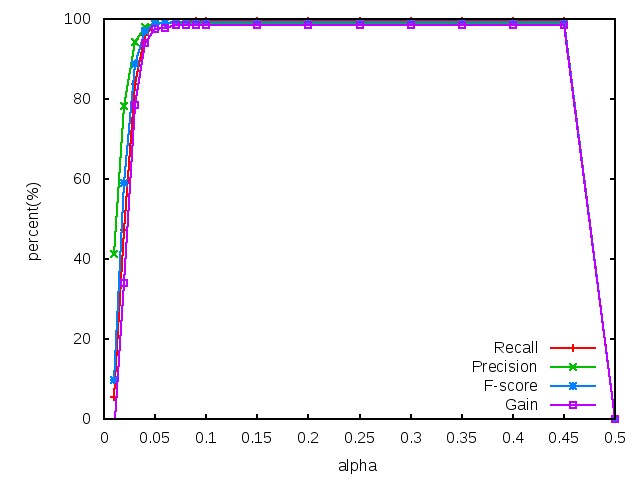
\includegraphics[width=0.5\textwidth]{alpha.jpg}
\caption{The effect of $\alpha$\label{fig:alpha}}
\end{center}
\end{figure}

If $\alpha$ is too small, too much solid kmers will be failed to get in table $A$ and too many positions will fail the hypothesis test. As a result, Lighter will try to correct those error-free region which also brings down the precision. And if $\alpha$ become even smaller, then there is no kmer in $B$, so Lighter will fail to correct all the reads because there is no candidate kmers. 

If $\alpha$ is larger, $y'$ will increase due to larger $\beta$ and the $f(\alpha)$ becomes constant when $\alpha>0.05$. As a result, it can handle this case nicely. However, when $\alpha$ is too large, the \kmer length $k$ will be smaller than $y'$, and all the positions will be regarded as untrusted. We can observe this from the dramatic drop in Figure \ref{fig:alpha}.

This explanation can also be verified by looking at the occupancy rate of table A and B from the simulated data sets with 3 different coverage and $1\%$ error rate when changing $\alpha$ shown in Figure \ref{fig:bloom_occupancy_alpha}. Also, we can see the occupancy rate of table A is almost the same given the same $\alpha\times\mbox{coverage}$ across the 3 data sets. And the occupancy rate of table B is very steady because the solid kmers from the genome are the same for the 3 data sets. 

\begin{figure}[h!]
\begin{center}
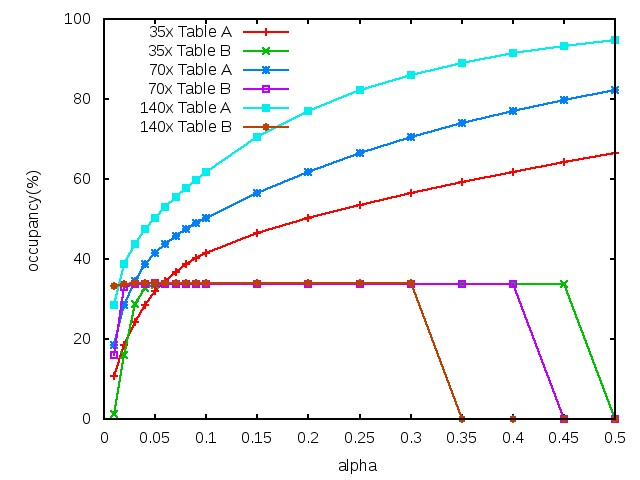
\includegraphics[width=0.5\textwidth]{bloom_occupancy_alpha.jpg}
\caption{The effect of $\alpha$ on occupancy rate\label{fig:bloom_occupancy_alpha}}
\end{center}
\end{figure}

\subsubsection*{Effect of kmer length}
One important parameters for \kmer based error correction methods is the value of $k$. When $k$ is too small, the \kmer containing sequencing error comes will likely be a \kmer from another location of the genome. When $k$ is too large, there may not be enough error-free \kmers for us to do error correction, especially when the coverage is not high. From the perspective of efficiency, when $k$ is large, we need more time to process a \kmer. And for the programs which requires storing the \kmer information, like using a hash table to store the counts, larger $k$ causes more memory consumption. Since Lighter does not store the \kmers' information explicitly, larger $k$ will only make Lighter slower but does not affect the memory usage.  In \cite{kelley2010quake}, the authors suggested that we can select $4^k$ around two hundred times the genome size. 

We measured the affect of $k$ using the simulated data set with $35 \times$ coverage and $1\%$ error rate, the result is shown in Figure \ref{fig:kmerLength}. 

\begin{figure}[h!]
\begin{center}
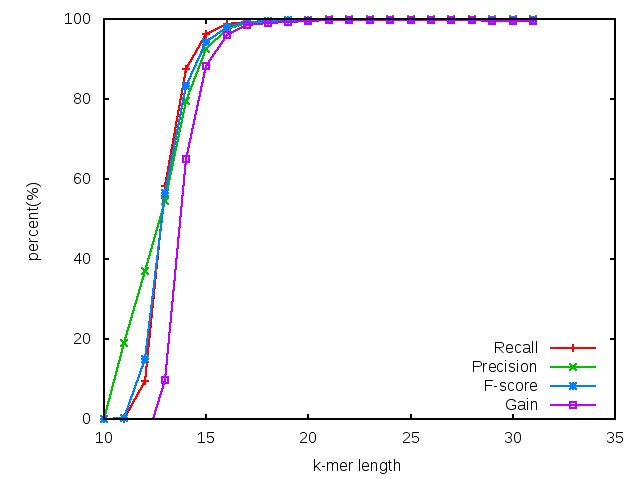
\includegraphics[width=0.5\textwidth]{kmerLength.jpg}
\caption{The effect of \kmer length\label{fig:kmerLength}}
\end{center}
\end{figure}


\subsection*{Real data set}
\subsubsection*{E.Coli data set}
We use ERR022075 data set which is a very deep coverage sequencing data set of ecoli K-12 strain genome. We still used Quake, Musket, Bless and Lighter to run this data set. Since usually we do not need that much of coverage, we uniformly sampled some reads from this data set and got a data set with roughly 75x coverage(total 3,497,616 reads). The reads in this data set is paired-end and the read length is 100 and 102. Because Bless can not handle paired-end reads with different length, we truncate the last 2 base to form a 100-length paired-end data set.

Since the genome of E.Coli K-12 strain is fully sequenced, we measured that 4,519,538 out of 4,553,699 kmers from the genome is stored in table $B$, which is more than $99\%$. This number can be slightly improved using larger $\alpha$. 
 
% Result of bowtie2
We can also measure the error corrections' effect on the alignment. We use Bowtie2[cite] to align the reads to the reference genome and count the total number of the matched position.

\begin{table}
\begin{tabular}{|c|c|c|c||c|c|} \hline
	 & \multicolumn{3}{|c||}{Read Level} & \multicolumn{2}{|c|}{Base Level} \\ \hline
     & Total Reads 	& Mapped Reads & Gain(\%) & Match/Read & Gain(\%) \\ \hline
Original & 3,497,616 & 	3,464,140	 & - & 99.038	& - \\ \hline
Quake	& 3,369,584	& 3,368,911	& -2.75	& 97.305	& -1.75  \\ \hline
Musket	& 3,497,616	& 3,467,878	& 0.11	& 99.601	& 0.57  \\ \hline
Bless	& 3,497,616	& 3,472,979	& 0.26	& 99.611	& 0.58  \\ \hline
Lighter	 & 3,497,616	&  3,476,425	& 0.35	& 99.611	& 0.58  \\ \hline

\end{tabular}
\caption{Alignment of E.Coli data set\label{table:ecoli_alignment}}
\end{table}

In this table, "Gain" means how much improvement for its previous column comparing with the original data set. Match/Read represents the average matched position against the reference genome for the mapped reads.

For Quake, the gain is negative mainly due to unreported reads and trimmed 3' end. It turns out Lighter gives the most improvement for both read level and base level.

For those reads not got trimmed and alinged to the genome without indels (cigar field like 100M in the SAM file), we measure the matched ratio for each position shown in Figure \ref{fig:ecoli_perbase}. Since many of the reads in this data set start with N, the first base's matching ratio of the original data set is very low. 

\begin{figure}[h!]
\begin{center}
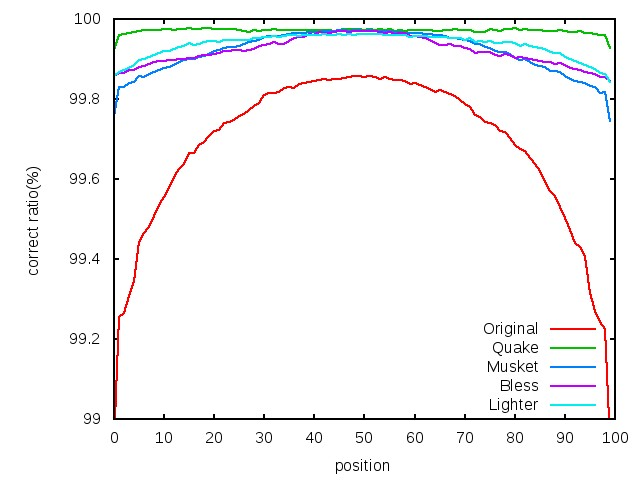
\includegraphics[width=0.5\textwidth]{per_base.jpg}
\caption{The matching ratio for each base in E.Coli data set\label{fig:ecoli_perbase}}
\end{center}
\end{figure}

% Result of Velvet
Another common measurement for error correction is to run the de novo assembly and see the impact to the contigs. We use Velvet[cite] to assemble the reads. Velvet is a de novo assembly software based on De Brujin graph. The parameter for Velvet especially the kmer size for the De Brujin graph is very important to the performance. We ran the Velvet on different parameters and choose the one with best N50 contig size for each program. Then for each chosen contig file, we evaluated the assembly quality using Quast[cite]. Since assemblers usually generates many very short contigs, we only choose the contigs whose length are no less than 100bp.

\begin{table}
\begin{tabular}{|c|c|c|c|c|c|} \hline
	 	& N50 &	NG50	 & Edits / 100kbps&	Misassemblies	& Coverage(\%) \\ \hline
Original	& 100,039	& 100,039	& 4.18	& 0	& 97.412 \\ \hline
Quake	& 125,252	& 125,252	& 4.23	& 8	& 97.450 \\ \hline
Musket	& 99,995	& 95,384	& 6.96	& 3	& 97.579 \\ \hline
Bless	& 104,682	& 99,991	& 4.45	& 3	& 97.352 \\ \hline
Lighter &	105,574	& 104,682	& 5.02	& 5	& 97.548 \\ \hline
\end{tabular}
\caption{De novo assembly of E.Coli data set\label{table:ecoli_assembly}}
\end{table}

N50 is the length such that the total length of the contigs longer or equal to than this length covers half of the assembled genome. And NG50 is the length of the contig with respect to the reference genome. Edits per 100kbps is the number of mismatches or indels per 100kbps when aligning the contigs to the reference genome. Misassembly is a position of a contig that its left sequence and right sequence are mapped far away on the genome or overlap too much. The coverage are the portion of the reference genome that are covered by contigs.

\subsubsection*{Human Chr14}
So far, we only tested the data on the genome of E.Coli, which is a pretty small. In this section, we use a data set from Gage[cite] on human chromosome 14. This data set is about 35x coverage and 101bp pair-end reads. And the \kmer size is 19 for all the programs in this data set.

Like for the E.Coli data set, we evaluate the result using both Bowtie2 and SOAPdenovo2.

The result of Bowtie2 is shown in Table \ref{table:chr14_alignment}.

\begin{table}
\begin{tabular}{|c|c|c|c||c|c|}\hline
  & \multicolumn{3}{|c||}{Read Level} & \multicolumn{2}{|c|}{Base Level} \\ \hline
  & Total Reads  & Mapped  &Gain(\%) &	Match/Read	& Gain(\%) \\ \hline
Original &	36,504,800	& 35,993,149	&- 		&	99.492	& - \\ \hline
Quake 	&	32,560,518	& 32,546,450	& -9.58 &	93.411	& -6.11 \\ \hline
Musket 	&	36,504,800 	&	36,276,990	& 0.79	& 100.104	& 0.62 \\ \hline
Bless 	&	36,504,800	&36,297,288	& 0.84	& 100.192	&	0.70 \\ \hline
Lighter	&   36,504,800	&36,280,350	& 0.80	& 100.109	& 0.62 \\ \hline
\end{tabular}
\caption{Alignment of chr14 data set\label{table:chr14_alignment}}
\end{table}

% Result of Velvet
We also tested the effect to de novo assembly using Velvet and Quast which is shown in Table \ref{table:chr14_assembly}. In this data set, the improvement due to error corrections is obviously. 

\begin{table}
\begin{tabular}{|c|c|c|c|c|c|} \hline
	   & N50 &	NG50	& Edits / 100kbps &	Misassemblies	& Coverage(\%) \\ \hline
Original &	8096 &5940	&134.53	&1097	&78.490 \\ \hline
Quake	& 7935	&5809	&143.91	&2110	&77.303 \\ \hline
Musket	& 6261	&4613	&128.97	&811	&78.984 \\ \hline
Bless	& 8397	&6201	&131.87 &1425	&78.747 \\ \hline
Lighter	& 8370	&6211	&133.22	&1416	&78.858 \\ \hline
\end{tabular}
\caption{De novo assembly of chr14 data set\label{table:chr14_assembly}}
\end{table}

The results of the de novo assembly of the two real data set show that Lighter's result is comparable with other methods.

\subsection*{Running Time and Space Usage}
%describe the machine
The programs were run on a machine with 48 2.1GHz processors, 512G memory and 74T disk space. 

%The memory or disk usage from different programs 
Musket, Bless and Lighter are all aimming for low memory consumption. So we compared the peak memory usage as well as the peak disk consumption on the simulated data set with different coverage and with $1\%$ error rate and the chr14 real data from Gage.

\begin{tabular}{|c|c|c||c|c||c|c||c|c|} \hline
		& \multicolumn{2}{|c||}{$35\times$} & \multicolumn{2}{|c||}{$70\times$}  & \multicolumn{2}{|c||}{$140\times$} & \multicolumn{2}{|c|}{chr14}  \\ \hline
		& memory & disk & memory & disk & memory & disk & memory & disk \\ \hline
Quake   & 2.8G	& 3.3G & 7.1G & 6.0G & 14G & 12G & 48G & 57G \\ \hline		
Musket	& 139M	& 0 & 160M & 0 & 241M & 0 & 1.9G & 0 \\ \hline
Bless	& 10M	& 661M & 11M & 1.3G & 13M & 2.6G & 600M & 15G \\ \hline
Lighter	& 31M	& 0 & 31M & 0 & 31M & 0 & 510M & 0 \\ \hline
\end{tabular}

From the table, we can see that Bless and Lighter can achieve nearly constant memory consumption as claimed. Musket took much less memory comparing with Quake but is much worse than Bless and Lighter.

For Bless, we increase the number of temporary files along with the coverage of the data set to achieve the constant memory consumption. Bless uses secondary memory to save the memory consumption, and the overall space consumption is much larger than Musket and Lighter.  For the chr14 data set, The memory consumption of Bless can be decreased if we create more temporary files. 

%runtime on simulated_70_1
We compared the running time between Quake, Musket and Lighter using different number of threads on the simulated data set with $70\times$ coverage and $1\%$ error in Figure \ref{fig:runtime}. Musket requires at least 2 threads due to its master-slave style parallelism, so its figure start at when number of threads is 2. 

\begin{figure}[h!]
\begin{center}
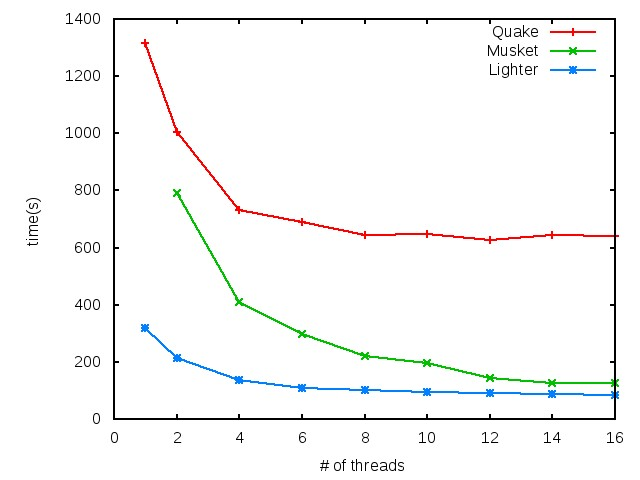
\includegraphics[width=0.5\textwidth]{runtime.jpg}
\end{center}
\caption{The running time on simulated data set with different number of threads\label{fig:runtime}}
\end{figure}

So far, Bless can only run in single-thread mode and it takes 1475s to finish which is much slower than Musket and Lighter.

The result shows that Lighter is very efficient and scalable. 

\section*{Discussion}
\tool is a software tool for correcting sequencing errors in sequencing datasets.
At \tool's core is a method for obtaining a set of solid \kmers from a large collection of sequencing reads.
Unlike previous methods, \tool does this without counting \kmers in the reads.
By setting its parameters appropriately, its memory usage and accuracy can be held almost constant with respect to depth of coverage.
It is also quite fast and practical.

Though we demonstrate \tool in the context of sequencing error correction, \tool's counting-free approach could be applied in other situation where a collection of solid \kmers is desired.
For example, one tool for scaling metagenome sequence assembly uses of a Bloom filter populated with solid \kmers as a memory-efficient, probabilistic representation of a De Bruijn graph \cite{pell2012scaling}.
Other tools use counting Bloom filters \cite{fan2000summary, bonomi2006improved} or the related CountMin sketch \cite{cormode2005improved} to represent De Bruijn graphs for compression \cite{jones2012compression} or digital normalization and related tasks \cite{zhang2013these}.
We expect Ideas from \tool could be useful in reducing the memory footprint of these and other tools. 

%We use this method to implement an error correction program Lighter for DNA-seq reads. As we expect, Light is space-efficient . Moreover, it is very fast and gives performance is comparable with other programs. This shows that our method of finding solid kmer is quite reliable. 

%Another immediate application of our method is getting solid kmers' count, which can be done by scanning the reads again to get the real count for the solid kmers stored in table $B$. 

%Since our method is probabilitic, we may miss few important information. Nevertheless, our method is extremely useful for programs like Quip[cite], where the accurate error correction is not critical. Even more, programs like Quip may directly use the solid kmers get by our method to do the assembly.

In this paper, we did not analyze the effect of $\alpha$ analytically and it is a difficult problem. So far, the size of table $A$ and $B$ are setting by considering unpractical pessimestic scenarios. If we know the effect in some compact form, we can optimize the performance of obtaining solid kmers by setting the best $\alpha$ and also use less space.

\tool is free open source software released under the XXX license.  The software and its source are available from \url{https://github.com/mourisl/Lighter/}.

%%%%%%%%%%%%%%%%%%%%%%%%%%%
\section*{Acknowledgements}
  Text for this section \ldots

\bibliographystyle{abbrv}
\bibliography{lighter_paper}

\end{document}







